\documentclass[11pt,a4paper]{article}

% Drop-in draft. Replace the preamble with the JOAS template when available;
% the body below uses only standard sectioning, tables and references.

\usepackage[utf8]{inputenc}
% Fontes vectorielles. Sans lmodern, l'encodage T1 avec les Computer Modern
% par defaut fait basculer LaTeX sur des fontes bitmap Type 3, et le PDF
% apparait pixelise a l'ecran comme a l'impression. lmodern fait partie de
% TeX Live et de MiKTeX ; si la distribution ne l'a pas, commenter la ligne
% suivante ET celle de fontenc plutot que de garder T1 seul.
\usepackage{lmodern}
\usepackage[T1]{fontenc}
\usepackage[margin=2.5cm]{geometry}
\usepackage{booktabs}
\usepackage{graphicx}
\graphicspath{{../figures/}{figures/}}
\usepackage{amsmath}
\usepackage{url}
\usepackage[hidelinks]{hyperref}
\usepackage{tikz}
\usetikzlibrary{arrows.meta, positioning, calc, backgrounds, fit, decorations.pathreplacing}
\definecolor{cNormal}{RGB}{70,90,110}
\definecolor{cSub}{RGB}{176,58,46}
\definecolor{cRoll}{RGB}{191,123,29}
\definecolor{cModel}{RGB}{47,84,150}
\definecolor{cOut}{RGB}{56,118,74}
\tikzset{
  dlabel/.style={font=\scriptsize, inner sep=1.5pt},
  dnote/.style={font=\scriptsize\itshape, align=left, inner sep=1.5pt},
  dbox/.style={draw, rounded corners=2.5pt, align=center, inner sep=5pt,
               minimum height=9mm, font=\small},
  dflow/.style={-{Latex[length=2.2mm]}, draw=black!50, line width=0.7pt},
  dspan/.style={-{Latex[length=2.2mm]}, line width=1.1pt},
  dband/.style={fill=black!3, rounded corners=3pt},
}
\usepackage{siunitx}
\sisetup{group-separator={,}}

\title{What Is a Taxi-Out Time?\\
Matching Windows, Silent Substitutions and a Generalist Model\\
for the PRC Data Challenge 2026}

\author{Ugo Roccamatisi\\
\small Centrale Lille and Cranfield University\\
\small Team \texttt{motivated-ostrich}}

\date{\today}

\begin{document}
\maketitle

\begin{abstract}
The PRC Data Challenge 2026 asks participants to predict taxi-out time for
departures at ten major European airports. Its final phase is a blind ranking
on four months of 2026, which rewards models that generalise rather than
models tuned on a public leaderboard. We describe the generalist model we
submitted and the analysis of the target that shaped it. The target is not
always a taxi time: about \SI{4.8}{\percent} of departures have their off-block
silently replaced by the scheduled time, and a rarer family carries a
date-rollover defect. We show that the airport off-block always lies within
\SI{3606}{\second} of the last filed off-block time, on all
\num{2062251} matched departures of 2025. This matching window bounds every
prediction and makes a schedule substitution impossible on a known subset of
flights; together these two consequences remove \SI{8.3}{\second} of error from
an earlier model. The final model is a two-regime mixture whose classifier,
regressors, mixture exponent and blend of CatBoost and per-airport XGBoost are
chosen on a selection fold and scored once on a separate control fold, without
leaderboard feedback. On January and July 2025 it reaches
\SI{348.3}{\second} of root mean squared error, against \SI{356.6}{\second}
for our earlier, partly leaderboard-tuned pipeline. A decomposition of the
remaining error shows that \SI{40}{\percent} of it sits in 26 aberrant labels
with no identifying signal and \SI{40}{\percent} in measurement noise on
ordinary flights, which no model restricted to the provided columns can
remove. We report the negative results that support this reading, including a
recalibration on EUROCONTROL's published monthly taxi-out times and a search
for co-occurring defects between arrivals and departures.
\end{abstract}

\section{Introduction}

Taxi-out time, the interval between off-block and takeoff, is a standard
efficiency indicator in air traffic management. It drives fuel burn and
associated emissions on the ground, it is a core metric of Airport
Collaborative Decision Making, and its predictability conditions departure
metering schemes. The literature on its prediction is mature: reported root
mean squared errors fall in the range of \SIrange{75}{90}{\second} on
carefully measured physical taxiing \cite{ravizza2014}, with queue
size at pushback consistently identified as the dominant predictor since
\cite{idris2001}.

The PRC Data Challenge 2026, organised by the EUROCONTROL Performance Review
Unit together with the OpenSky Network, provides twelve months of 2025
movement data at ten European airports. The initial phase ranked predictions
for January and July 2026 on a public leaderboard. Shortly before the end, the
organisers added a final phase: a single blind submission on a new file
covering January, February, June and July 2026 (\num{670790} departures), with
no leaderboard, together with a review of code and documentation. The stated
reason was that signs of optimisation against the public ranking had become
too strong.

This change of rules is the frame of the present paper. Our public score with
the second-campaign pipeline was \SI{319.21}{\second}, in the lower half of a
leaderboard then led at \SI{241.75}{\second}, and several of its settings had been
selected or confirmed with leaderboard feedback. For the final phase we
rebuilt the model from scratch under one constraint: every setting is chosen
on 2025 data, with a selection fold and a separate control fold, and every
component rests either on a structural property of the data or on that
out-of-time validation.

We organise the paper around five claims.

\begin{enumerate}
\item The target is not always a taxi time, and its two corrupted families
behave completely differently with respect to prediction: one is recomputable
from provided columns, the other has no identifying signal in any field or
signature we tested (Section~\ref{sec:anatomy}).
\item The airport off-block never leaves a \SI{\pm 3606}{\second} window
around the last filed off-block time. This structural property bounds every
prediction and rules out schedule substitution on a known subset of flights
(Section~\ref{sec:window}).
\item A generalist model selected without leaderboard feedback outperforms,
on the same holdout, our earlier pipeline that was partly tuned on the
leaderboard, and the gain of
each selected component transfers from the selection fold to the control fold
(Sections \ref{sec:method} and \ref{sec:results}).
\item Most of the remaining error is not reducible with the provided columns:
it sits in a few aberrant labels and in the disagreement between two
off-block definitions (Section~\ref{sec:floor}).
\item Congestion features are screened off by the observed Network Manager
off-block, but only in the causal direction, which reflects the difference
between forecasting and retrospective reconstruction
(Section~\ref{sec:direction}).
\end{enumerate}

All code, the Kaggle notebook that produced the final submission, the
complete experiment log with both positive and negative results, and the
diagnostics that support every number in this paper are available at
\url{https://github.com/ugo-roccamatisi/prc-data-challenge-2026}.

\section{Data and task}
\label{sec:data}

The challenge provides \num{4167797} movements, arrivals and departures, at
EDDF, EDDM, EGLL, EHAM, LEBL, LEMD, LFPG, LIRF, LSZH and LTFM for the whole of
2025. Each movement record carries the reporting airport's own timestamps: the
movement time (takeoff for a departure, landing for an arrival), the block
time (off-block or in-block), the scheduled time, and the stand and runway
used. Movement records are left-joined onto the Network Manager flight list,
which contributes the flight plan and flown trajectory timestamps, in
particular the last filed off-block time (LOBT), the estimated off-block time
(EOBT) and the actual off-block time of the flown trajectory (AOBT).

In the ranking files, only two fields are blanked, and only for departures:
the block time and the taxi time. Everything else remains visible, including
the takeoff time, the scheduled time, the stand, the runway, every Network
Manager field, and all arrival records with their in-block times and taxi-in
durations. The organisers confirmed that the Network Manager columns are
admissible inputs in the final phase.

About \SI{1.5}{\percent} of departures are never matched to a Network Manager
record, in which case every flight-side column is null. For matched flights,
the airport off-block and the Network Manager off-block do not measure the
same event. The naive estimator \(\widehat{y} = \text{MVT} - \text{AOBT}\)
gives a root mean squared error of \SI{380.8}{\second} over the whole of 2025,
with a per-airport hourly median bias ranging from \SI{-118}{\second} at LIRF
to \SI{+296}{\second} at LTFM (Figure~\ref{fig:bias}). This is not noise
around a common definition; it is two definitions. Our models therefore
predict the residual of the target over that naive estimator rather than the
target itself.

\begin{figure}[t]
\centering
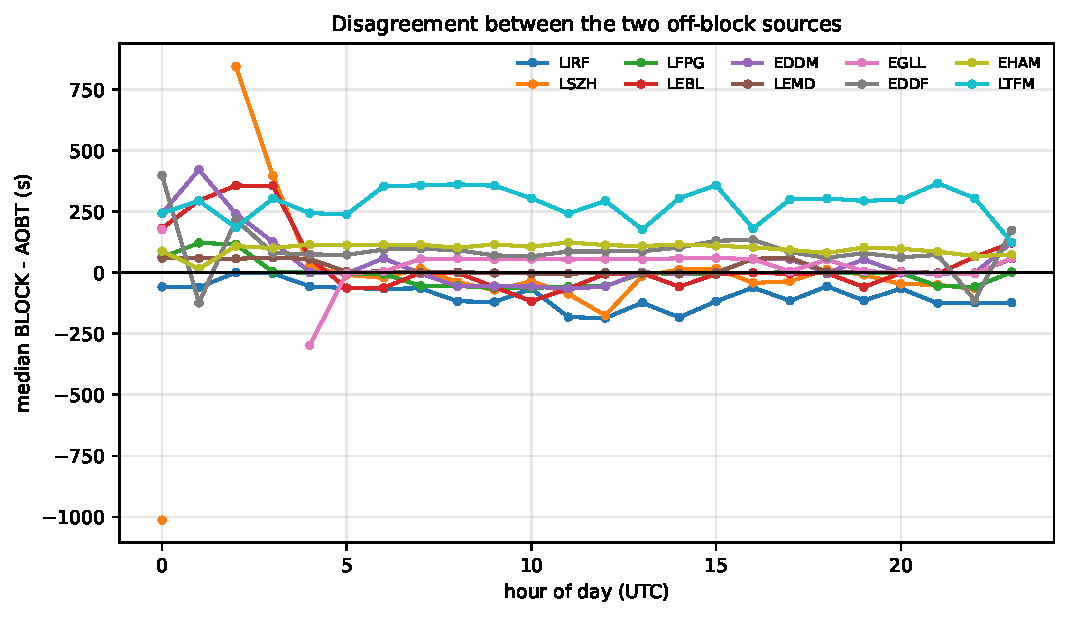
\includegraphics[width=0.85\textwidth]{fig1_offblock_bias.pdf}
\caption{Hourly median of the difference between the airport block time and
the Network Manager actual off-block, per airport, 2025. The curves do not
scatter around a common zero: the two sources measure different events, and
the per-airport offset reaches several minutes.}
\label{fig:bias}
\end{figure}

\section{Anatomy of the target}
\label{sec:anatomy}

\begin{figure}[t]
\centering
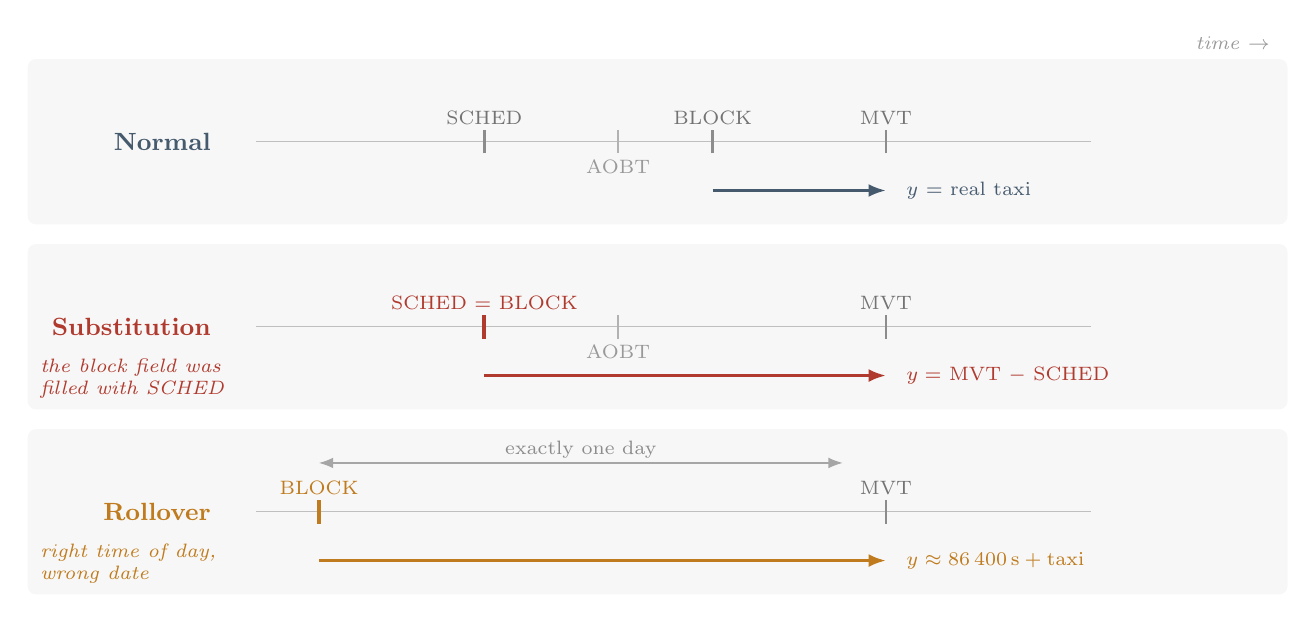
\begin{tikzpicture}[font=\small]
\def\W{10.6}
\def\SC{2.9}  \def\AO{4.6}  \def\BL{5.8}  \def\MV{8.0}
\def\RH{1.55}

% ---- bandes de fond, une par regime
\foreach \i in {0,1,2}{
  \fill[dband] (-2.9,-\i*2.35+1.05) rectangle (\W+2.5,-\i*2.35-1.05);
}

% ============ 1. enregistrement normal
\begin{scope}
  \node[anchor=east, font=\small\bfseries, text=cNormal] at (-0.45,0) {Normal};
  \draw[draw=black!25] (0,0) -- (\W,0);
  \foreach \x/\t in {\SC/SCHED, \BL/BLOCK, \MV/MVT}{
    \draw[draw=black!45, line width=0.9pt] (\x,-0.15) -- (\x,0.15);
    \node[dlabel, above, text=black!55] at (\x,0.16) {\t};
  }
  \draw[draw=black!30, line width=0.9pt] (\AO,-0.15) -- (\AO,0.15);
  \node[dlabel, below, text=black!40] at (\AO,-0.17) {AOBT};
  \draw[dspan, cNormal] (\BL,-0.62) -- (\MV,-0.62);
  \node[dlabel, anchor=west, text=cNormal] at (\MV+0.2,-0.62) {$y$ = real taxi};
\end{scope}

% ============ 2. substitution de l'heure programmee
\begin{scope}[yshift=-2.35cm]
  \node[anchor=east, font=\small\bfseries, text=cSub] at (-0.45,0) {Substitution};
  \draw[draw=black!25] (0,0) -- (\W,0);
  \draw[draw=cSub, line width=1.4pt] (\SC,-0.15) -- (\SC,0.15);
  \node[dlabel, above, text=cSub] at (\SC,0.16) {SCHED $=$ BLOCK};
  \draw[draw=black!30, line width=0.9pt] (\AO,-0.15) -- (\AO,0.15);
  \node[dlabel, below, text=black!40] at (\AO,-0.17) {AOBT};
  \draw[draw=black!45, line width=0.9pt] (\MV,-0.15) -- (\MV,0.15);
  \node[dlabel, above, text=black!55] at (\MV,0.16) {MVT};
  \draw[dspan, cSub] (\SC,-0.62) -- (\MV,-0.62);
  \node[dlabel, anchor=west, text=cSub] at (\MV+0.2,-0.62) {$y =$ MVT $-$ SCHED};
  \node[dnote, anchor=north west, text=cSub] at (-2.8,-0.35)
    {the block field was\\filled with SCHED};
\end{scope}

% ============ 3. decalage d'un jour
\begin{scope}[yshift=-4.70cm]
  \node[anchor=east, font=\small\bfseries, text=cRoll] at (-0.45,0) {Rollover};
  \draw[draw=black!25] (0,0) -- (\W,0);
  \draw[draw=cRoll, line width=1.4pt] (0.8,-0.15) -- (0.8,0.15);
  \node[dlabel, above, text=cRoll] at (0.8,0.16) {BLOCK};
  \draw[draw=black!45, line width=0.9pt] (\MV,-0.15) -- (\MV,0.15);
  \node[dlabel, above, text=black!55] at (\MV,0.16) {MVT};
  \draw[{Latex[length=1.8mm]}-{Latex[length=1.8mm]}, draw=black!35]
    (0.8,0.62) -- node[dlabel, above, text=black!45] {exactly one day} (\MV-0.55,0.62);
  \draw[dspan, cRoll] (0.8,-0.62) -- (\MV,-0.62);
  \node[dlabel, anchor=west, text=cRoll] at (\MV+0.2,-0.62)
    {$y \approx \SI{86400}{\second} + {}$taxi};
  \node[dnote, anchor=north west, text=cRoll] at (-2.8,-0.35)
    {right time of day,\\wrong date};
\end{scope}

\node[font=\scriptsize\itshape, text=black!40, anchor=east] at (\W+2.4,1.25)
  {time $\rightarrow$};
\end{tikzpicture}
\caption{The three regimes of the target, drawn on a common time axis with the
takeoff aligned. In a normal record the reported taxi time spans the airport
block time to takeoff. Under schedule substitution the block field carries the
scheduled time, so the reported value is the departure delay plus the taxi, and
is exactly recomputable from two columns that remain visible at evaluation
time. Under date rollover the block field carries the correct time of day with
the previous day's date, which inflates the value by one day and leaves no
visible trace.}
\label{fig:regimes}
\end{figure}


\subsection{Schedule substitution}

Selecting departures for which the recorded block time equals the scheduled
time to within \SI{10}{\second} isolates \SI{4.80}{\percent} of departures. On
those rows the recorded taxi time is, to within a median of \SI{3}{\second},
exactly \(\text{MVT} - \text{SCHED}\): the reported quantity is the sum of the
departure delay and the real taxi, not the taxi. The median recorded value is
\SI{1009}{\second} against \SI{910}{\second} for the rest of the population,
so the contamination is invisible in a summary statistic
(Figure~\ref{fig:substitution}), but these rows carry \SI{29}{\percent} of the
total squared error of a naive regression. The organisers document that they
did not reconcile inconsistencies between the movement and flight sources,
which is consistent with what we observe: the substitution is an artefact of
the reporting chain, left in place by design.

\begin{figure}[t]
\centering
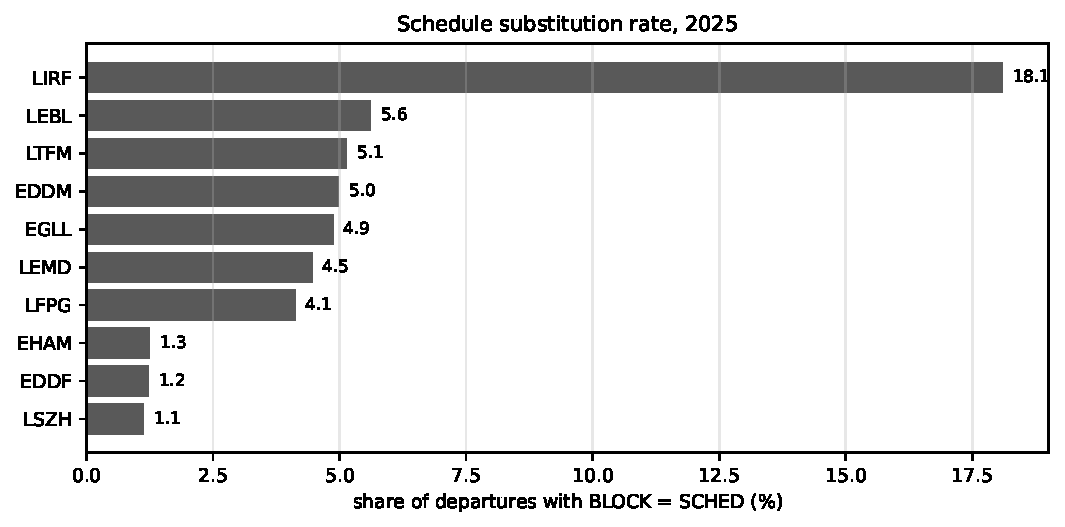
\includegraphics[width=0.85\textwidth]{fig2_substitution_rate.pdf}
\caption{Share of departures whose recorded block time equals the scheduled
time to within \SI{10}{\second}, per airport, 2025. On those rows the reported
taxi time is the departure delay plus the real taxi.}
\label{fig:substitution}
\end{figure}

\subsection{A recomputable subfamily}
\label{sec:rule}

Among the substituted rows, the extreme tail is the one that matters for a
squared-error metric. In 2025 there are \num{76} departures with a recorded
taxi time above \SI{20000}{\second}. Of these, \num{58} satisfy
\(\lvert y - (\text{MVT} - \text{SCHED})\rvert < \SI{120}{\second}\), and
\num{72} are at LIRF. On those rows \(y - (\text{MVT} - \text{SCHED})\) has a
median of \SI{1}{\second} and an interquartile range of \SI{6}{\second}.

Since both the takeoff time and the scheduled time remain visible in the
ranking file, these labels are recomputable rather than predictable. The
difficulty is identification. A threshold on \(\text{MVT} - \text{SCHED}\)
alone is a poor discriminator: at \SI{20000}{\second} it selects \num{245}
candidates for \num{57} true positives. The discriminating conjunction
involves the join structure rather than the timestamps: requiring in addition
that the movement be unmatched to any Network Manager record and that the
aircraft type field be empty raises precision from \num{0.23} to \num{0.85}.

In the second campaign we applied this rule as a hard substitution restricted
to LIRF, worth \SI{7.95}{\second} on the leaderboard. The final model keeps the
identification but not the airport restriction or the hard decision: for
unmatched movements without aircraft type whose \(\text{MVT} - \text{SCHED}\)
exceeds \SI{3}{\hour}, the label equals \(\text{MVT} - \text{SCHED}\) on
\SI{67}{\percent} of the \num{244} such departures of 2025, and the prediction
uses that rate, estimated per airport and shrunk towards the global rate, as a
mixture weight (Section~\ref{sec:method}).

\subsection{A family without a usable identifier}
\label{sec:rollover}

The remaining \num{18} aberrant labels of 2025 follow a different mechanism.
Fourteen of them lie between \SI{87168}{\second} and \SI{88392}{\second}, that
is \SI{86400}{\second} plus an ordinary taxi: the recorded block time carries
the correct time of day and the previous day's date. The quantity
\(y - \SI{86400}{\second}\) matches a planned delta on one row out of
eighteen, and \(\text{MVT} - \text{SCHED}\) on these rows ranges from
\SI{939}{\second} to \SI{93535}{\second}, so no threshold isolates them.

We tested a second hypothesis for the final phase. Arrivals in the ranking
file keep their labels, and the same defect appears on arrivals. If the
defect were a property of the reporting system on a given night, buggy
arrivals would point at the nights where departures are at risk. On 2025, no
departure defect lies within \SI{24}{\hour} of an arrival defect at the same
airport (the nearest is \SI{27}{\hour} away), the result is identical when the
arrivals are shifted by \(\pm 7\) days as a placebo, and the pure one-day
arrival defect occurs twice in 2025 and never in the 2026 ranking file. The
defect is per flight, not per night. We therefore make no correction for this
family. This is an empirical statement about the fields and signatures we
tested, not a proof that identification is impossible.

\section{The matching window}
\label{sec:window}

The Network Manager flight list carries several off-block clocks. For every
departure matched to it in 2025, the airport block time lies within
\SI{3606}{\second} of the last filed off-block time:
\begin{equation}
\lvert \text{BLOCK} - \text{LOBT} \rvert \le \SI{3606}{\second}
\quad\text{on \num{2062251} of \num{2062251} matched departures.}
\label{eq:window}
\end{equation}
The other clocks satisfy the same bound on \SI{99.997}{\percent} (IOBT),
\SI{99.97}{\percent} (EOBT) and \SI{99.91}{\percent} (AOBT) of rows, and the
sharp edge of the distribution (Figure~\ref{fig:window}) identifies the bound
as the tolerance of the join between the two sources rather than a property of
operations. A movement whose off-block falls outside the window is simply not
matched.

\begin{figure}[t]
\centering
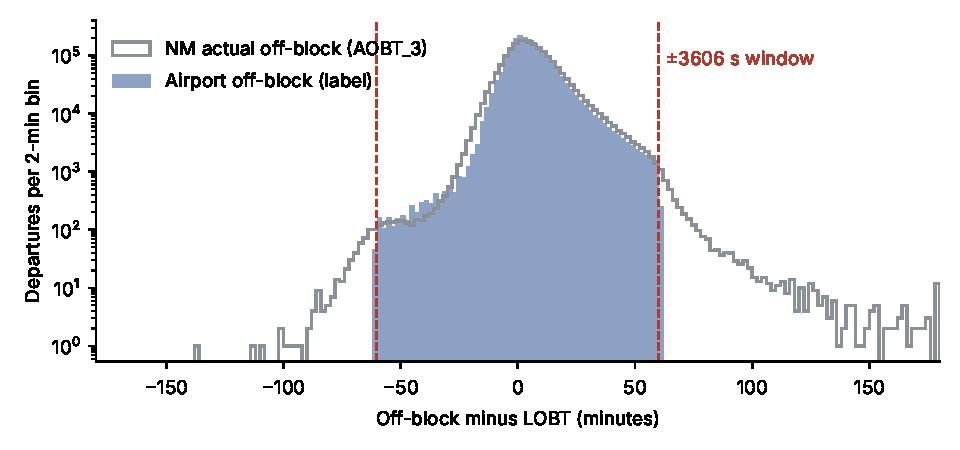
\includegraphics[width=0.9\textwidth]{fig5_lobt_window.pdf}
\caption{Distance between the off-block and the last filed off-block time,
2025 departures matched to the Network Manager, logarithmic scale. The airport
off-block, which defines the label, stops exactly at \(\pm\SI{3606}{\second}\);
the Network Manager actual off-block does not.}
\label{fig:window}
\end{figure}

Equation~\eqref{eq:window} has two consequences, and both can only reduce the
error.
\begin{enumerate}
\item The true taxi time lies in
\([\text{MVT} - \text{LOBT} - 3606,\ \text{MVT} - \text{LOBT} + 3606]\).
Projecting any prediction on that interval brings it closer to the truth or
leaves it unchanged.
\item A schedule substitution writes SCHED into the block field. It is
therefore impossible when \(\lvert \text{SCHED} - \text{LOBT} \rvert >
\SI{3606}{\second}\). In the January and July 2025 holdout, \num{13869}
departures are in that case and none of them is substituted, yet a classifier
that ignores the bound still assigns them a positive substitution probability,
weighted by delays that can reach several hours.
\end{enumerate}
Applied after the fact to the holdout predictions of an earlier pipeline (v15),
the projection alone reduced the root mean squared error from
\SI{345.0}{\second} to \SI{340.7}{\second}, and setting the substitution
probability to zero on infeasible rows brought it to \SI{336.7}{\second}.
Neither step involves a learnt parameter.

\section{Method}
\label{sec:method}

\subsection{Model}

Because the target mixes regimes, a single conditional-mean regressor is badly
misspecified: we measured \SI{472.8}{\second} for a single model against
\SI{379.1}{\second} for a mixture on an identical feature set in an earlier
campaign. The final model (Figure~\ref{fig:pipeline}) predicts
\begin{equation}
\widehat{y} = \Pi_{\text{LOBT}}\Bigl[\,p^{\gamma}\,(\text{MVT} - \text{SCHED})
 + \bigl(1 - p^{\gamma}\bigr)\,\mu\,\Bigr],
\label{eq:model}
\end{equation}
where \(\Pi_{\text{LOBT}}\) is the projection on the matching window and the
components are as follows.

\begin{itemize}
\item \(p\) is a global XGBoost classifier for schedule substitution, trained
only on departures where substitution is feasible, and set to zero elsewhere.
\item \(\mu\) is the normal-regime taxi. When the Network Manager off-block
gives a plausible taxi, \(0 \le \text{MVT} - \text{AOBT} \le
\SI{7200}{\second}\), regressor A predicts the residual over it; otherwise
regressor B predicts the taxi directly. Both are trained on non-substituted
labels between \SI{30}{\second} and \SI{7200}{\second}, and \(\mu\) is clipped
to that range.
\item The exponent \(\gamma\) reflects that a squared loss rewards the
expectation over the two regimes, not the most likely regime; it is chosen on
the selection fold (\(\gamma = 0.9\)).
\item For unmatched movements without aircraft type and with
\(\text{MVT} - \text{SCHED} > \SI{3}{\hour}\), \(p^{\gamma}\) is replaced by
the substitution rate of that subset in the training data
(Section~\ref{sec:rule}).
\end{itemize}

Three families are trained for regressors A and B: global XGBoost,
per-airport XGBoost for regressor A (all ten airports exceed the size
threshold of \num{40000} rows), and global CatBoost with native categorical
handling. Their weights, on a grid of step \num{0.25}, and the exponent are
chosen jointly on the selection fold, with an eligibility rule fixed in
advance: a blend must beat XGBoost alone by at least \SI{0.5}{\second},
otherwise XGBoost alone is kept. The selected blend is \num{0.75} CatBoost and
\num{0.25} per-airport XGBoost. The final model is trained on the twelve
months of 2025 with \num{1.1} times the number of trees found by early
stopping, three seeds averaged.

\begin{figure}[t]
\centering
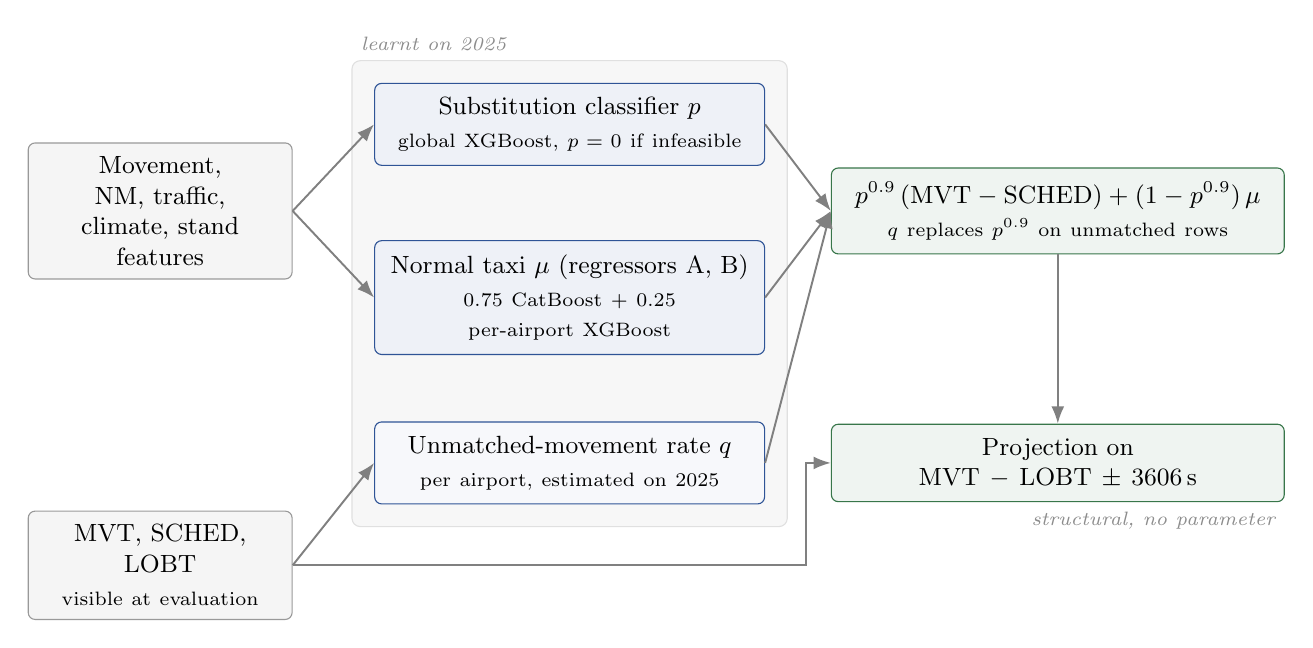
\begin{tikzpicture}[
  font=\small,
  inp/.style={dbox, fill=black!4, draw=black!40, text width=30mm},
  mdl/.style={dbox, fill=cModel!8, draw=cModel, text width=46mm},
  res/.style={dbox, fill=cOut!8, draw=cOut, text width=54mm},
]
\node[inp] (feat)  at (0,1.6)  {Movement, NM, traffic,\\climate, stand features};
\node[inp] (lobt)  at (0,-2.9) {MVT, SCHED, LOBT\\[1pt]\scriptsize visible at evaluation};

\node[mdl] (clf) at (5.2,2.7)
  {Substitution classifier $p$\\[1pt]\scriptsize global XGBoost, $p=0$ if infeasible};
\node[mdl] (reg) at (5.2,0.5)
  {Normal taxi $\mu$ (regressors A, B)\\[1pt]\scriptsize 0.75 CatBoost $+$ 0.25 per-airport XGBoost};
\node[mdl, fill=cModel!4] (rule) at (5.2,-1.6)
  {Unmatched-movement rate $q$\\[1pt]\scriptsize per airport, estimated on 2025};

\node[res] (mix) at (11.4,1.6)
  {$p^{0.9}\,(\text{MVT}-\text{SCHED}) + (1-p^{0.9})\,\mu$\\[1pt]\scriptsize $q$ replaces $p^{0.9}$ on unmatched rows};
\node[res] (proj) at (11.4,-1.6)
  {Projection on\\$\text{MVT}-\text{LOBT}\pm\SI{3606}{\second}$};

\draw[dflow] (feat.east) -- (clf.west);
\draw[dflow] (feat.east) -- (reg.west);
\draw[dflow] (clf.east)  -- (mix.west);
\draw[dflow] (reg.east)  -- (mix.west);
\draw[dflow] (rule.east) -- (mix.west);
\draw[dflow] (lobt.east) -- (8.2,-2.9) -- (8.2,-1.6) -- (proj.west);
\draw[dflow] (lobt.east) -- (rule.west);
\draw[dflow] (mix.south) -- (proj.north);

\begin{scope}[on background layer]
\node[dband, draw=black!12, fit=(clf)(reg)(rule), inner sep=8pt] (stage) {};
\end{scope}
\node[font=\scriptsize\itshape, text=black!45, anchor=south west]
  at (stage.north west) {learnt on 2025};
\node[font=\scriptsize\itshape, text=black!45, anchor=north east]
  at (proj.south east) {structural, no parameter};
\end{tikzpicture}
\caption{The final model. The substitution classifier, the regressors and the
unmatched-movement rate are learnt on 2025; the feasibility condition and the
projection follow from the matching window and have no parameter. The blend
weights and the exponent are chosen on the selection fold.}
\label{fig:pipeline}
\end{figure}

\subsection{Features}

Departure labels (block time and taxi time) are masked in the training data
before any contextual feature is built, so that training features are
computed under exactly the conditions of the ranking file. The feature set has
six groups: plan and clock deltas (takeoff minus each of SCHED, AOBT, LOBT,
EOBT and IOBT, the Network Manager delay, the feasibility flag, the day gap);
traffic around the takeoff (departures and arrivals within
\SI{15}{\minute}, same-runway departures \SI{10}{\minute} before and
\SI{5}{\minute} after, gaps to the neighbouring takeoffs); an off-block
anchored queue (aircraft taxiing at the flight's off-block, takeoffs between
its off-block and its takeoff, recent Network Manager taxi times); the
airport climate of the hour and of the day (mean Network Manager taxi and
delay, arrival taxi-in, arrival substitution rate); the previous arrival at
the same stand; and categorical identifiers (airport, runway, stand, aircraft
type, destination, operator, market segment, wake category), plus a stand and
runway reference of the Network Manager taxi computed on the training fold.
The traffic and climate windows are symmetric around the takeoff, so they
include some later movements, but the dedicated posterior sequence features of
our second campaign are excluded; the reason is given in
Section~\ref{sec:direction}.

\subsection{Validation protocol}

Two folds are built on 2025. The selection fold trains on all months except
January, April, July and October and validates on April and October; it sets
the number of trees by early stopping, the exponent and the blend weights. The
control fold trains on all months except January and July, validates on
January and July, mimicking the seasonality of the ranking set, and is scored
once with the settings of the selection fold. Nothing is chosen on the control
fold, and nothing in the final model is chosen with leaderboard feedback.

\section{Results}
\label{sec:results}

Table~\ref{tab:families} gives the selection and control scores of each
regressor family and of the selected blend. The blend gained \SI{5.9}{\second}
over XGBoost alone on the selection fold; on the control fold it gains
\SI{6.7}{\second} overall and \SI{8.9}{\second} on the clean lane, labels up to
\SI{20000}{\second}. Both exceed the \SI{2.9}{\second} range we measured
across three seeds of one configuration (Section~\ref{sec:noise}). On this
problem CatBoost alone outperforms XGBoost alone, as it outperformed LightGBM
in our second campaign, which we attribute to its ordered target statistics on the
high-cardinality stand and operator variables.

\begin{table}[t]
\centering
\caption{Root mean squared error (seconds) of each regressor family and of
the selected blend. The selection fold chose the blend; the control fold is
scored once. The clean lane excludes labels above \SI{20000}{\second}.}
\label{tab:families}
\begin{tabular}{lrrr}
\toprule
& Selection & Control & Control, clean lane \\
& Apr + Oct & Jan + Jul & Jan + Jul \\
\midrule
Second-campaign pipeline (v26) & & 356.60 & 259.19 \\
XGBoost & 221.92 & 355.00 & 271.70 \\
Per-airport XGBoost & 221.44 & 354.15 & 270.59 \\
CatBoost & 217.22 & 348.99 & 263.65 \\
\textbf{0.75 CatBoost + 0.25 per-airport} & \textbf{216.06} & \textbf{348.29} & \textbf{262.76} \\
\bottomrule
\end{tabular}
\end{table}

The gain is spread over all ten airports (Table~\ref{tab:airports}). Against
the second-campaign pipeline, the final model is \SI{8.3}{\second} better
overall and \SI{3.6}{\second} worse on the clean lane. The clean-lane gap is
consistent with the posterior sequence features we left out, worth
\SI{3.3}{\second} on the clean lane of the holdout when they were introduced.

\begin{table}[t]
\centering
\caption{Clean-lane root mean squared error (seconds) per airport and month,
control fold, XGBoost alone and selected blend.}
\label{tab:airports}
\begin{tabular}{lrrrr}
\toprule
& \multicolumn{2}{c}{January 2025} & \multicolumn{2}{c}{July 2025} \\
\cmidrule(lr){2-3}\cmidrule(lr){4-5}
Airport & XGBoost & Blend & XGBoost & Blend \\
\midrule
EDDF & 176.9 & 174.3 & 198.4 & 191.0 \\
EDDM & 180.7 & 170.5 & 187.1 & 179.8 \\
EGLL & 248.0 & 239.0 & 307.8 & 292.0 \\
EHAM & 210.1 & 199.9 & 175.6 & 168.2 \\
LEBL & 144.8 & 140.7 & 268.2 & 262.5 \\
LEMD & 162.9 & 155.9 & 191.7 & 185.9 \\
LFPG & 271.3 & 257.6 & 260.1 & 247.7 \\
LIRF & 329.2 & 321.3 & 710.4 & 697.8 \\
LSZH & 218.9 & 212.1 & 205.5 & 197.6 \\
LTFM & 228.4 & 221.5 & 290.3 & 276.3 \\
\bottomrule
\end{tabular}
\end{table}

Table~\ref{tab:ablation} isolates the structural components. The unmatched
rule is worth \SI{6.3}{\second} on the selection fold and \SI{44.3}{\second}
on the control fold, because July 2025 carries many unmatched LIRF rows with
large delays: it is the component with the largest variance across months, and
its contribution to the final score depends on how often the defect occurs in
2026. The projection is worth \SI{1.3}{\second} and \SI{5.3}{\second}.

\begin{table}[t]
\centering
\caption{Ablation of the structural components of the selected model, root
mean squared error in seconds.}
\label{tab:ablation}
\begin{tabular}{lrr}
\toprule
Model & Selection & Control \\
\midrule
Full model & 216.06 & 348.29 \\
Without the unmatched-movement rule & 222.40 & 392.55 \\
Without the rule and the projection & 223.71 & 397.87 \\
\bottomrule
\end{tabular}
\end{table}

The final submission was produced on a Kaggle T4 GPU in about \SI{4.8}{\hour},
of which CatBoost takes most. The \num{670790} identifiers of the submission
template all match departures of the final ranking file.

\section{How much of the remaining error is reducible?}
\label{sec:floor}

Table~\ref{tab:anatomy} decomposes the squared error of the control fold by
regime. The proportions come from a reduced run on \SI{60}{\percent} of the
training rows (\SI{359.9}{\second} overall) and match those of the full run.

\begin{table}[t]
\centering
\caption{Decomposition of the control-fold mean squared error by regime.}
\label{tab:anatomy}
\begin{tabular}{p{4.2cm}rrp{5.4cm}}
\toprule
Regime & Rows & Share of MSE & Reducible with the provided columns? \\
\midrule
Labels above \SI{20000}{\second} & 26 & \SI{40}{\percent} & No identifying signal found \\
Normal departures & \num{323650} & \SI{40}{\percent} & Measurement noise \\
Unmatched to the Network Manager & \num{5227} & \SI{15}{\percent} & At most 10 points, with a perfect classifier \\
Schedule substitution & \num{15324} & \SI{5}{\percent} & Classifier plateaus at AUC 0.88 \\
\bottomrule
\end{tabular}
\end{table}

Twenty-six rows weigh as much as \num{323650} ordinary flights. A single
defective record of the rollover family contributes roughly \num{21500} to the
mean squared error of a two-month validation set; with about twelve such
events a year, a two-month evaluation window is a Poisson draw, and the
ranking of two models separated by a few seconds is partly decided by it.

On the normal lane, the model regresses towards the mean: taxis below
\SI{10}{\minute} are over-predicted by about \SI{100}{\second} and taxis of
30 to \SI{60}{\minute} are under-predicted by about \SI{400}{\second}. This is
the signature of an error in the conditioning variable rather than of a
missing regressor. The disagreement between the airport and Network Manager
off-blocks has a per-airport standard deviation between \SI{250}{\second} and
\SI{500}{\second}; our clean-lane error of \SI{263}{\second} is roughly twice
the \SIrange{75}{90}{\second} reported in the literature on cleanly measured
taxiing. Under a squared loss, shrinkage towards the mean is the optimal
response to such noise, and a different model fed the same columns cannot
undo it. The information that could, a physical observation of the
push-back, is not in the provided data: surface ADS-B tracks are the obvious
candidate, and we did not use them.

For the unmatched movements, a perfect substitution classifier on that lane
would remove 10 of its 15 points of squared error, an upper bound that no
realistic classifier approaches. We conclude that the large remaining gains
lie outside the provided columns, and we do not claim that the remaining gap
to the leading models is irreducible with external data.

\section{Directionality of the congestion screening}
\label{sec:direction}

The strongest predictor in the taxi-time literature is the state of the
departure queue at pushback \cite{idris2001, ravizza2014}. We implemented it
twice, in two independent forms: queue length and recent throughput anchored
on the aircraft's own off-block, and a demand queue counting flights whose
planned pushback preceded the takeoff without having departed. Both were
neutral to slightly negative. The explanation is conditioning: once the
Network Manager off-block is observed, the model already knows the duration of
the flight's own ground phase as measured by the second source, and the queue
that produced that duration adds nothing.

\begin{figure}[t]
\centering
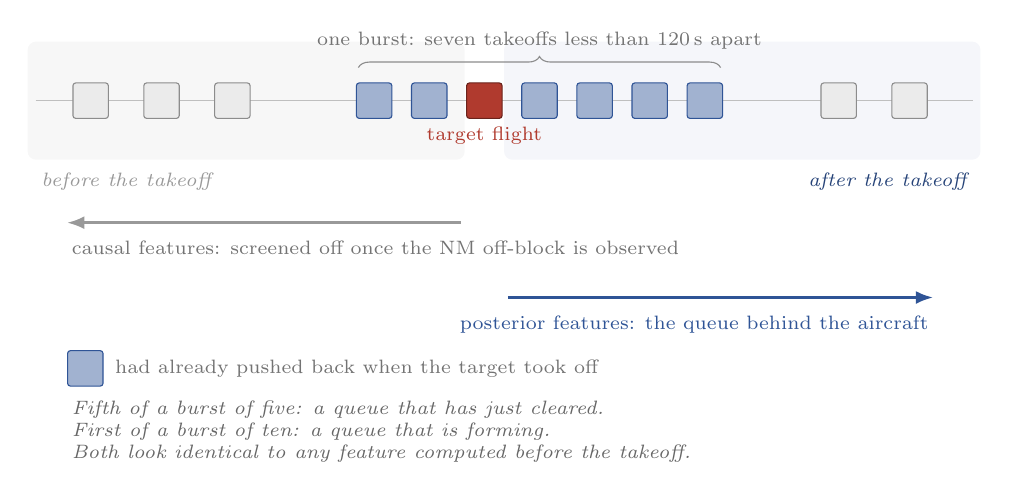
\begin{tikzpicture}[
  font=\small,
  dep/.style={draw=black!45, fill=black!8, minimum width=4.5mm,
              minimum height=4.5mm, inner sep=0pt, rounded corners=1pt},
  tgt/.style={dep, fill=cSub, draw=cSub!60!black},
  behind/.style={dep, fill=cModel!45, draw=cModel},
  brace/.style={decorate, decoration={brace, amplitude=4pt}, draw=black!45},
]
\def\T{5.9}
\fill[black!3, rounded corners=3pt] (0.1,-0.75) rectangle (\T-0.25,0.75);
\fill[cModel!5, rounded corners=3pt] (\T+0.25,-0.75) rectangle (12.2,0.75);
\node[font=\scriptsize\itshape, text=black!40, anchor=north west] at (0.15,-0.8)
  {before the takeoff};
\node[font=\scriptsize\itshape, text=cModel!80!black, anchor=north east]
  at (12.15,-0.8) {after the takeoff};

\draw[draw=black!25] (0.2,0) -- (12.1,0);

\foreach \x/\sty in {0.9/dep, 1.8/dep, 2.7/dep, 4.5/behind, 5.2/behind,
                     5.9/tgt, 6.6/behind, 7.3/behind, 8.0/behind, 8.7/behind,
                     10.4/dep, 11.3/dep}{
  \node[\sty] at (\x,0) {};
}
\node[dlabel, text=cSub, anchor=north] at (\T,-0.28) {target flight};
\draw[brace] (4.3,0.42) -- node[above=5pt, dlabel, text=black!55]
  {one burst: seven takeoffs less than \SI{120}{\second} apart} (8.9,0.42);

\draw[{Latex[length=2.2mm]}-, draw=black!40, line width=1pt]
  (0.6,-1.55) -- (\T-0.3,-1.55);
\node[dlabel, text=black!55, anchor=north west] at (0.6,-1.72)
  {causal features: screened off once the NM off-block is observed};

\draw[-{Latex[length=2.2mm]}, draw=cModel, line width=1pt]
  (\T+0.3,-2.5) -- (11.6,-2.5);
\node[dlabel, text=cModel, anchor=north east] at (11.6,-2.67)
  {posterior features: the queue behind the aircraft};

\node[behind, anchor=west] at (0.6,-3.4) {};
\node[dlabel, text=black!55, anchor=west] at (1.15,-3.4)
  {had already pushed back when the target took off};
\node[dnote, text=black!60, anchor=north west] at (0.6,-3.75)
  {Fifth of a burst of five: a queue that has just cleared.\\
   First of a burst of ten: a queue that is forming.\\
   Both look identical to any feature computed before the takeoff.};
\end{tikzpicture}
\caption{Why the congestion screening is directional. Each square is a takeoff
on the same runway. Features computed from earlier takeoffs add nothing once
the Network Manager off-block is observed, because that timestamp already
encodes the queue the aircraft went through. Features computed from later
takeoffs, in particular the count of subsequent departures that had already
left their stand, measure the queue the aircraft was part of, and no causal
feature can substitute for them.}
\label{fig:direction}
\end{figure}


The screening is directional, however. The ranking file contains every
movement of the evaluation months, including the departures that took off
after the target flight. Features built from those (intervals to the next
takeoffs on the same runway, the position of the flight within a burst of
closely spaced takeoffs, and above all the number of the next ten departures
that had already pushed back when the target took off) gained
\SI{3.62}{\second} on the leaderboard in our second campaign and improved
eight airports out of ten on the holdout. That last feature is the queue
behind the aircraft, and it is measurable only by looking forward.

These features have no operational meaning. A controller does not know future
takeoffs, and a model using them cannot be deployed for departure metering.
They are admissible in a retrospective reconstruction task, which is what the
challenge is, but they change what a reported score means. For the final
model we left out these dedicated forward-looking features, keeping only
symmetric traffic and climate windows around the takeoff, at an estimated cost
of about \SI{3}{\second} on the clean lane. We
believe the distinction between forecasting and reconstruction is worth making
explicit in challenge design, since it silently changes the admissible
feature space.

\section{Negative results and measured variability}
\label{sec:noise}

\subsection{What did not work}

Table~\ref{tab:negative} lists the substantive ideas we tested and rejected
across the three campaigns. We report them because several are ideas a reader
would otherwise be likely to try.

\begin{table}[t]
\centering
\caption{Rejected hypotheses. Effects are on 2025 validation data unless
stated otherwise.}
\label{tab:negative}
\begin{tabular}{p{7.2cm}p{7.2cm}}
\toprule
Hypothesis & Outcome \\
\midrule
Recalibrate airport-month means on EUROCONTROL's published monthly taxi-out
times & Model means already within \SI{20}{\second} of the truth; the series
differs from the labels by up to \SI{166}{\second} in winter. Costs
\SIrange{0.7}{3.1}{\second} out of time \\
Flag rollover defects through arrival defects on the same night & No
co-occurrence; placebo at \(\pm 7\) days identical \\
Expectation correction for the rollover family, calibrated on 2025 rates &
\SI{+19.8}{\second} on holdout, \SI{-2.45}{\second} on the leaderboard \\
Single regressor instead of the regime mixture & Costs \SI{94}{\second} \\
Queue and throughput features anchored on pushback & Neutral, twice \\
Demand queue anchored on scheduled and estimated off-block & \SI{-1.6}{\second} \\
Degraded-day detection from arrival taxi-in & No effect: a de-icing aircraft
delays itself, not the arrivals \\
Meteorological features (temperature, dew-point spread, precipitation codes)
& Degraded July: temperature acts as a season surrogate \\
Upper clipping of predictions & Degrades at every threshold: the extreme
labels are real \\
Open ADS-B derived off-block times (OPDI) & Ground coverage between
\SI{0.2}{\percent} and \SI{16}{\percent}; first detection trails the off-block
by \SIrange{700}{1300}{\second} \\
\bottomrule
\end{tabular}
\end{table}

The recalibration deserves a note. EUROCONTROL publishes, per airport and
month, the number of departures and the total reference and additional
taxi-out time, from which a mean taxi-out follows, including for the months of
the final file. In spring and summer this mean agrees with the mean of our
clean labels within about \SI{15}{\second} at eight airports out of ten; in
winter it lies \SIrange{50}{166}{\second} below them
at EDDF, EDDM, LFPG and LSZH, a gap consistent with de-icing being counted
differently. Our model's airport-month means were already within
\SI{20}{\second} of the truth on the control fold, so shifting them towards
the published series made predictions worse. A published aggregate is only a
useful anchor if its definition matches the label.

The rollover correction teaches a related lesson. It was validated by a
month-transfer protocol within 2025, improved both validation months, and
still lost on the leaderboard: with about twelve events a year, a two-month
window does not estimate a rate. Modelling a data defect from its historical
frequency assumes the producing system is statistically stationary at the
evaluation scale, an assumption that is not testable within the data.

\subsection{How large is a real effect?}

In our second campaign, three seeds of a single fixed configuration gave
\SI{366.43}{\second}, \SI{366.17}{\second} and \SI{363.52}{\second}, a range of
\SI{2.9}{\second}. Three runs do not estimate a variance, and random training
and data partitioning are known to produce non-negligible performance
variation in model comparisons \cite{raste2022}; we use the range as a warning
threshold. It renders several of our own earlier single-seed comparisons
unresolved. The components of the final model clear it with margin: the blend
gains \SI{6.7}{\second} on a fold where it was not selected, and the
structural components of Section~\ref{sec:window} involve no learnt parameter.

\section{Earlier campaigns}
\label{sec:history}

The final model is the third of three campaigns. The first built the regime
mixture and selected its exponent on the leaderboard over the grid
\(\{0.5, 0.6, 0.75, 1.0\}\); the public and holdout curves were parallel with
an offset of about \SI{32}{\second} (Figure~\ref{fig:gamma}), our first
evidence that holdout gains transfer for physical properties of the model.
The second campaign added the reconstruction rule, the posterior sequence
features, per-airport regressors with a global classifier and a CatBoost
ensemble; Table~\ref{tab:leaderboard} traces its public progression. Because
several of those settings were chosen or confirmed with repeated leaderboard
queries, which can overfit a public leaderboard \cite{blum2015}, we treat
these gains as descriptive. The third campaign kept the ideas that rest on
structure or on out-of-time validation and re-selected every setting on 2025.

\begin{figure}[t]
\centering
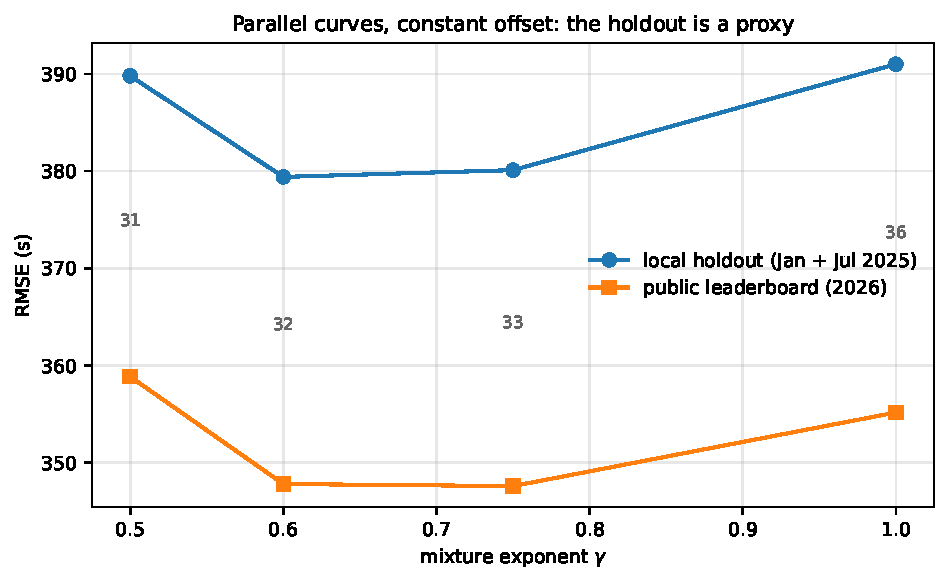
\includegraphics[width=0.7\textwidth]{fig4_gamma_transfer.pdf}
\caption{Holdout and public root mean squared error as a function of the
mixture exponent \(\gamma\), first campaign. The two curves are parallel with
an offset of about \SI{32}{\second}.}
\label{fig:gamma}
\end{figure}

\begin{table}[t]
\centering
\caption{Public leaderboard progression of the second-campaign pipeline. Each
row adds one change to the row above.}
\label{tab:leaderboard}
\begin{tabular}{llr}
\toprule
Submission & Change & Public RMSE (s) \\
\midrule
v19 & Merged baseline pipeline & 338.37 \\
v21 & Label reconstruction rule (Section~\ref{sec:rule}) & 330.42 \\
v22 & Posterior sequence features (Section~\ref{sec:direction}) & 326.80 \\
v23 & Double capacity, lean classifier, three-seed average & 325.15 \\
v25 & Per-airport regressors, global classifier, CatBoost & 320.10 \\
v26 & CatBoost weight \num{0.75} & \textbf{319.21} \\
\bottomrule
\end{tabular}
\end{table}

\section{Discussion}

\subsection{Implications for operational data}

Two major terms in our residual are produced by the reporting chain: the
disagreement between two off-block definitions, and defects whose provenance
is hidden. For the data producers, publishing a provenance flag alongside the
block time, a substitution indicator where the scheduled time was used as a
fallback, and a boolean recording that a date was inferred rather than
observed would be worth more than any modelling applied downstream. The
matching window of Section~\ref{sec:window} illustrates the converse: a single
documented property of the join removed more error than most of the modelling
changes we tried.

\subsection{Limitations}

CatBoost reached its iteration cap in the selection fold (\num{6000} trees for
regressor A, \num{4000} for regressor B) without triggering early stopping,
so the final blend is likely slightly under-trained. February and June are in
the final file but not in a validation fold; they exist in the 2025 training
data and lie seasonally between the two folds. The unmatched-movement rule
depends on the frequency of an airport-side defect and its contribution varies
widely between months. The error decomposition of Table~\ref{tab:anatomy}
comes from a reduced run. Our evaluation rests on months of 2025 as a proxy for
months of 2026, which cannot detect non-stationarity of the kind that defeated
the rollover correction, and we had no access to the systems that produce the
block times, so our characterisation of the defects is inferred from their
traces.

\subsection{Reproducibility}

The repository provides the final pipeline as a single script
(\texttt{src/taxiout\_general.py}) and as the Kaggle notebook that produced
the submission, with fixed seeds. A run writes the selected settings, the
fold scores and the out-of-fold predictions of both folds. The full run takes
about \SI{4.8}{\hour} on a Kaggle T4 GPU, and \SI{17}{\minute} with XGBoost
alone. The final model uses only challenge data. The diagnostics behind the
counts of Sections~\ref{sec:anatomy} and~\ref{sec:window}, the co-occurrence
test, the complete experiment log and the earlier pipelines are kept in the
repository; the challenge data are not redistributed.

\section{Conclusion}

The taxi-out times distributed in this challenge are, for a small but decisive
fraction of departures, not taxi-out times. We characterised two families of
defects, recovered one from visible columns and found no identifier for the
other. We showed that the airport off-block never leaves a one-hour window
around the last filed off-block, a property of the join that bounds every
prediction and rules out substitution on a known subset of flights at no
modelling cost. On that basis we built a generalist model selected without
leaderboard feedback, which outperforms our earlier leaderboard-tuned pipeline
on the same holdout and whose selected components transfer from one
validation fold to another. Most of the error that remains lies in a few
unidentifiable records and in the disagreement between two off-block
definitions; reducing it further calls for new information, such as a
physical observation of the push-back, rather than a different model of the
same columns.

\section*{Acknowledgements}

We thank the EUROCONTROL Performance Review Unit and the OpenSky Network for
assembling and releasing the dataset and for running the final blind phase,
and the participants of the challenge forum for the public discussion of
validation protocols and leaderboard probing.

\begin{thebibliography}{9}

\bibitem{idris2001}
Idris, H., Clarke, J.-P., Bhuva, R., and Kang, L.,
``Queuing Model for Taxi-Out Time Estimation,''
\emph{Air Traffic Control Quarterly}, Vol.~10, No.~1, 2002.

\bibitem{ravizza2014}
Ravizza, S., Chen, J., Atkin, J. A. D., Burke, E. K., and Stewart, P.,
``Aircraft Taxi Time Prediction: Comparisons and Insights,''
\emph{Applied Soft Computing}, Vol.~14, 2014, pp.~397--406,
doi:10.1016/j.asoc.2013.10.004.

\bibitem{blum2015}
Blum, A., and Hardt, M.,
``The Ladder: A Reliable Leaderboard for Machine Learning Competitions,''
\emph{Proceedings of the 32nd International Conference on Machine Learning},
Vol.~37, 2015, pp.~1006--1014.

\bibitem{raste2022}
Raste, S., Singh, R., Vaughan, J., and Nair, V. N.,
``Quantifying Inherent Randomness in Machine Learning Algorithms,''
arXiv:2206.12353, 2022, doi:10.48550/arXiv.2206.12353.

\end{thebibliography}

\end{document}
